%#########
%#Event generation
%#########
\par As discussed in Section~\ref{sec:qcdTheory}, theoretical interpretation of physical processes depends
 on the energy scales at which they occur. Processes during and after a $pp$ collision occur at a 
wide range of energy scales, from the \TeV\ to the \MeV\ scale.   
The factorization theorem~\cite{Collins:1989gx} fortunately enables separation of cross section calculations at high 
energy scales from those at low energy scales. The separation is encoded in the factorization 
factor $\mu_F(Q)$ which is a function of the energy scale $Q$. For $pp$ collisions 
at the LHC $Q$ is taken to be such that the produced system can be contained in a radius of just 
below a femtometer. Theories at these energy scales are then renormalized according to the 
renormalization group~\cite{Sonoda:2006rr}. The renormalization is encoded in the parameter $\mu_R$ which, as discussed 
in Section~\ref{sec:qcdTheory} is a function of the coupling constant $\alpha_S$. The production cross section 
of a system $X$ in a $pp$ collision is then formulated as  

\begin{equation}
\sigma_{pp\to X} = \sum_{a,b}\int dx_adx_bf_a(x_a,\mu_F^2)f_b(x_b,\mu_F^2)\times\sigma_{ab\to X}(x_ap_a,x_bp_b,\mu_F^2,\mu_R^2)
\label{eq:xs}
\end{equation}

The functions $f_a(f_b)$ are the Parton Distribution Functions (PDFs) that describe the probability of a parton of 
flavor $a(b)$ to have fraction $x_a(x_b)$ of the proton momentum $p_a(p_b)$ at an energy scale determined by $\mu_F$.
Since QCD cannot predict all the partons in a proton, PDF shapes are obtained by fitting their ad-hoc analytical forms to 
experimental data. Some of the groups that maintain these PDFs are CTEQ~\cite{Kovarik:2013sya}, 
NNPDF~\cite{Ball:2013hta}, HERAPDF~\cite{Kretzschmar:2009ws}, and MSTW~\cite{Watt:2012np}. 
Figure~\ref{fig:pdfs} shows an example of PDFs obtained from several the MSTW group. 

\begin{figure}[h]
   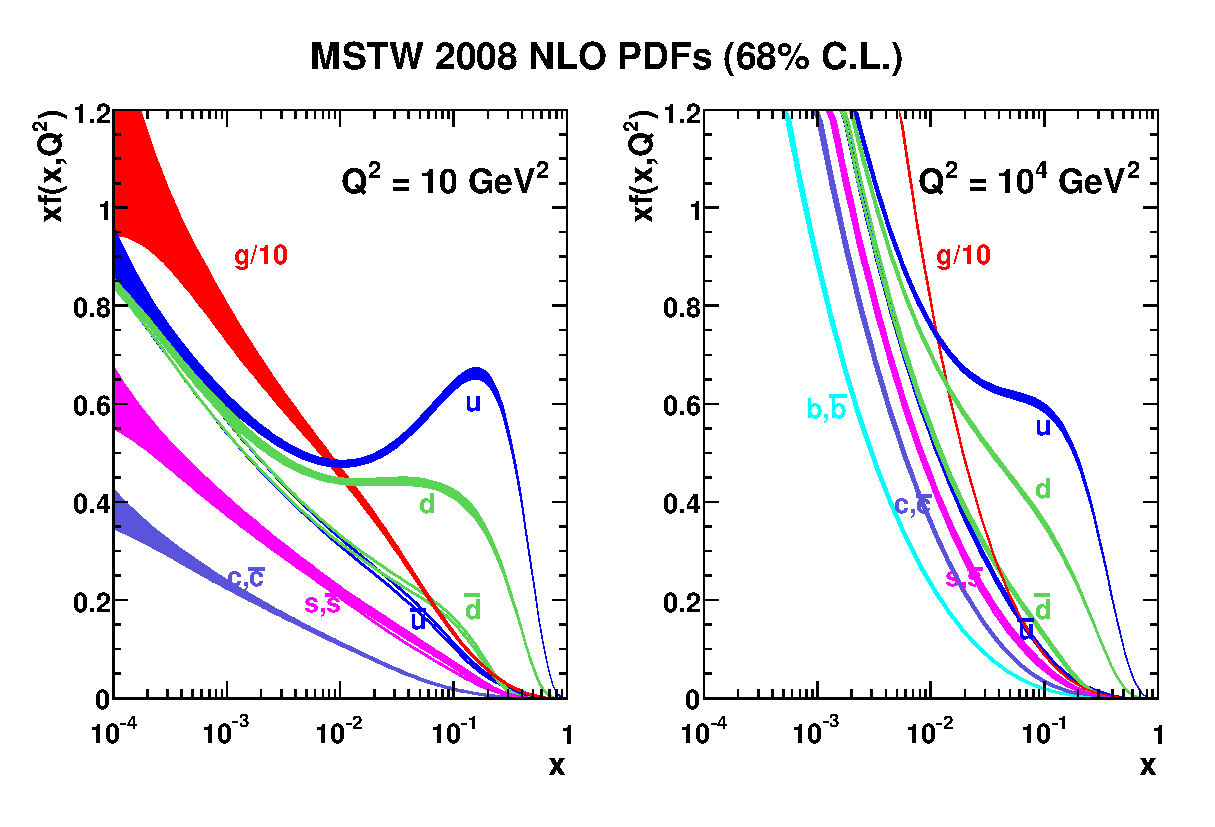
\includegraphics[width=\textwidth]{figures/mstw2008nlo68cl_allpdfs.eps}
\caption{Parton distribution functions obtained from the MSTW group. 
This image was obtained from Ref.~\cite{Martin:2009iq}}
\label{fig:pdfs}
\end{figure}

$\sigma_{ab\to X}$ is the parton level production cross section for system $X$. 
The process $ab\to X$ is known as the `hard scatter'. The cross section depends on 
$\mu_R^2$, and can be expanded into Equation~\ref{eq:partXS}.

\begin{equation}
\hat{\sigma}_{ab\to X} = \sum_{k=0}^{\infty}\int d\Phi_{X+k}|\sum_{l=0}^{\infty}\mathcal{M}_{X+k}^l|^2
\label{eq:partXS}
\end{equation}

$\mathcal{M}_{X+k}^l$ is a matrix element that encodes the amplitude of the process $ab\to X+k$, where $k$ 
are the additional partons in the final state. The index $l$ indicates the number of additional 
corrections to the process, colloquially known as `loops'. Essentially, $k$ represents real emmisions from 
the production in the sense that the additional final state partons alter the final state configuration of the 
process, and $l$ represents 
virtual emmisions because the final state remains unchanged. The leading order (LO) matrix element for production of $X$
is $\mathcal{M}_X^0$ while the LO matrix element for production of $X+k$ is $\mathcal{M}_{X+k}^0$. $l=1$ is 
known as next to leading order (NLO) and $l=2$ is next to next to leading order (NNLO). During simulation, the sum in 
Equation~\ref{eq:partXS} is normally truncated, at NNLO at best. The matrix elements are integrated over the phase 
space of the $X+k$ system and the integral is summed over an infinite number of final state partons. This sum is
in practice also truncated after a few terms. 

\par Divergences may arise in the cross section when two final state partons become collinear or when a final state 
parton becomes collinear with an initial state parton. They may also happen when a final state parton emits a gluon 
with such a small transverse momentum that the resulting gluon and the parton have an indistinguishable angular separation. 
The former are known as collinear emissions and the latter as soft emissions. The probability for a parton to not split or 
emit another parton, that may cause divergences, is encoded in the Sudakov form factor~\cite{Collins:1989bt}. It will be referred to 
frequently in later sections.
Virtual corrections from loops $l$ also cause divergences. The KLN theorem~\cite{Grandou:1994rz} however guarantees that at any order, 
divergences from virtual corrections cancel divergences from collinear splitting and soft emissions. So,
 $\hat{\sigma}_{ab\to X}$ remains accurate up to high order correction pertubations.   

\par To generate a heavy system through an elastic $pp$ collision the KMR model, introduced 
in Section~\ref{sec:exclH}, is used. Without loss of generality, the system discussed here is the Higgs boson system, 
and the process is referred to as the exclusive Higgs process. 
The collision occurs at a relatively smaller energy scale, $\mu_F^2\sim m_H$, than the energy scale 
for inelastic collisions. Consequently, formulation of the corresponding cross section takes a slightly
different approach than Equation~\ref{eq:xs}, and is encoded in 

\begin{equation}
\sigma_{pp(gg)\ra ppH} \propto \hat{\sigma}(gg\ra H)\left ( \int \frac{dQ^2_t}{Q^4_t}f_g(x_1, x_1^{'},Q^2_t, \mu_F^2)f_g(x_2, x_2^{'},Q^2_t, \mu_F^2)\right )^2 
\end{equation}

where $\hat{\sigma}(gg\ra H)$ is the parton-level cross-section
for the gluon fusion process that produces the Higgs boson, which is 
calculated at LO using matrix elements introduced above.  
The functions $f_g$ are the generalized gluon densities. These are a non-trivial 
combination of the gluon PDFs and the Sudakov form factor. The Sudakov 
form factor is introduced because the process of interest is that in which 
the initial state gluons do not radiate any other gluons. The generalized gluon 
densities take $x_1,x_2$, which are equivalent to Equation~\ref{eq:xs}'s $x_a,x_b$, 
and the factorization scale $\mu_F^2$ as inputs.   
The variables $x_1^{'}$ and $x_2^{'}$ are the fractions 
of the momentum carried by the exchanged third gluon with respect to the momenta of
protons $P_1$ and $P_2$.
Finally, the gluon densities are integrated over the exchanged (third) gluon 
transverse momentum $Q_t$. Figure~\ref{fig:exclHa} illustrates the production of the exclusive 
Higgs boson, with labels of the parameters discussed above.  

\begin{figure}[!h]
\centering
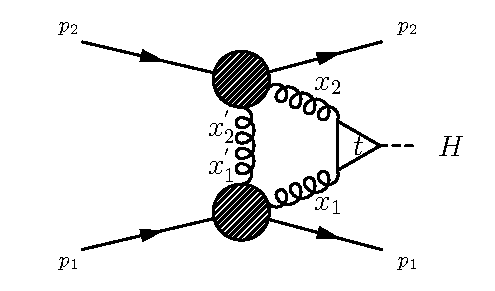
\includegraphics[width=0.8\linewidth]{figures/exclH.pdf}
\caption{Feynman diagram for the exclusive Higgs boson production} 
\label{fig:exclHa}
\end{figure}

\subsection{Parton Shower Development}
\label{sec:partonShower}
\par In simulation, shower development is achieved by pertubatively expanding on the hard scatter process. 
For a $pp$ collision with $k$ final state partons and differential cross section $d\sigma_{k}$,
the differential cross section of a process with $k+1$ final state partons is 
 
\begin{equation}
d\sigma_{k+1} = d\sigma_{k}\times\frac{\alpha_S(t)}{2\pi}P_{a,bc}(z)\frac{dt}{t}dz\frac{d\phi}{2\pi}
\label{eq:part}
\end{equation}

where the additional parton is obtained from a split or emission from one of the $k$ partons, which 
for reference can be called the `original parton'.
In the multiplicative factor, $t$ is the energy of the original parton, $z$ is the fraction of 
the energy carried by the additional parton in relation to $t$, and $\phi$ is the angular separation 
between the additional and the original partons. $P_{a,bc}$ is the probability that a parton of flavor 
$a$ splits or transforms into partons of flavor $b$ and $c$. So during simulation, given an energy scale $t$, Equation~\ref{eq:part} 
is sampled and partons are emitted at an energy scale $t^{'}$. If $t^{'}$ is below a threshold scale, the shower 
developement is terminated. Otherwise, the process is repeated recursively for each parton.
The threshold for $t^{'}$ known as the infrared cut-off, and it is about 1~\GeV. Figure~\ref{fig:pshower} 
shows a schematic of a parton shower developed in this manner.

\subsection{Hadronization}
\label{sec:hadronization}
\par Hadronization is the process that occurs immediately following the parton shower, when colored 
partons combine to form color-singlet hadrons. These hadrons are 
dominated by pseudoscalar and vector mesons, and spin-$1/2$ and spin-$3/2$ baryons.
They are referred to as primary hadrons, and the hadrons that they decay to 
are referrred to as secondary hadrons. The hadronization energy scale by construction 
is equal to the infrared cut-off of the parton shower. Phenomenological models are implemented 
in several event generators to describe hadronization, the most common being 
the {\it string} and {\it cluster} models. 

\par The string model utilizes the observation from lattice QCD~\cite{Gupta:1997nd} that the potential between a color 
charge dipole grows linearly with the distance, $r$, between the two charges. The Coulomb potential from the 
electric charge, being inversely proportional $r$, is negligible at large $r$.   
In the model, the potential between the two partons is represented by a quasi-elastic string 
that holds the two partons together. As $r$ grows, it may become more favorable to produce a 
$\qqbar$ pair from the vacuum than to maintain a tight string. Each of the parton in the \ttbar\ 
pair attaches itself to one of the partons in the original dipole through a new string, essentially 
doubling the number of dipoles in the system. Gluons can also be created from the vacuum as loops or 
`kinks' on the string, and may subsequently split into a \qqbar pair. Mass or flavor of the produced 
quarks and gluons is determined by the energy in the string breakup process. Because $c$ and $b$ quarks are 
heavy, they are rarely produced at the infrared cut-off scale $(\sim 1~\GeV)$. 
Baryons are produced when pairs of di-quarks are formed during the string break-up, instead of a 
\qqbar.

\par The main idea behind the cluster model is that gluons at the end of the parton shower 
are forced to split to \qqbar\ pairs. The flavor of these \qqbar\ pairs is determined by the 
gluon energy. Again $\bbbar$ and $\ccbar$ are rarely produced at the 1~\GeV\ energy scale. 
After the forced splits, a set of color-singlet hadrons is obtained by clustering pairs of 
quarks. Heavy singlets are allowed to decay to lighter ones at this stage. The formed clusters, in general, 
are regarded as excited mesons because they by construction will comprise two partons. 
They eventually decay to other hadrons that are more stable, including baryons.     

\par All these particles are saved in a record that documents their production, decays and splits. 
This record is known as the `truth' record. 

\subsection{Underlying Event and Pileup}
\par Apart from the primary hard scatter partonic interaction, additional activity is more often than not observed 
within a $pp$ collision. This additional activity is collectively referred to as the {\it underlying event}.
The underlying event is dominated by additional partonic interactions. 
These additional interactions introduce additional parton showers in the event. 
These showers 
lower the resolution for measuring observables for the primary event, so they eventually have to be corrected for.
Event generators are available that account for the underlying event and they are tuned 
to match what is observed in data.  

\par Additional activity from other $pp$ collisions within the same bunch is called {\it in-time pileup}, otherwise 
it is called {\it out-of-time pileup}. During Run I of the LHC, on average 20.7 extra $pp$ collisions 
from pileup were observed. During Run II, this number was even larger. Pileup is factored into the simulated event during 
the detector simulation part of the chain, as will be discussed in Section~\ref{sec:detsim}. 

\par Figure~\ref{fig:pshower} illustrates the development of both the hard scatter event and 
a secondary event, which contributes to pileup events. The red blob in the figure represents the 
hard scatter event sorrounded by parton showers and other particles 
undergoing Brehmsstrahlung. The purple blob similarly represents the secondary pileup event. 
The light green blobs represent hadronization. The hadrons formed decay to the dark green blobs which 
continually decay until stable final state particles are reached. The yellow lines represent 
soft photon radiation.  

\begin{figure}[!h]
   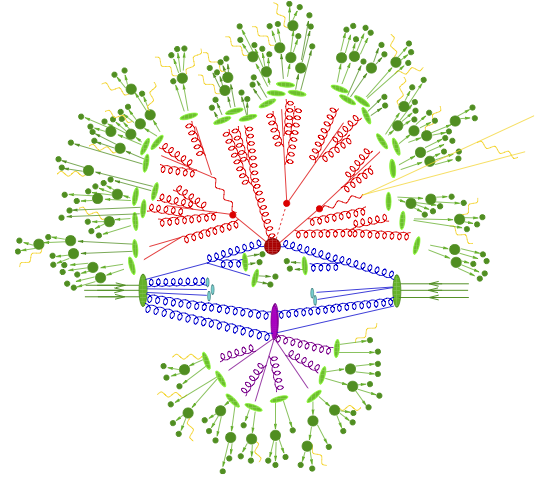
\includegraphics[width=\textwidth]{figures/pShower.png}
\caption{An illustration of the parton shower development, hadronization and hadron decays. 
Taken from Ref~\cite{Hoche:2014rga}}
\label{fig:pshower}
\end{figure}

\subsection{Monte Carlo Generators}
\par \PYTHIAsix~\cite{Pythia6} is the standard event generator for ATLAS.
Written in FORTRAN, it generates the hard scatter event at LO and implements the parton showering 
and hadronization models. Event generation uses both hard and soft scale models, so it is able to 
generate the underlying event as well. Its parameters were tuned to fit ATLAS conditions. 
A similar generator called \PYTHIA8~\cite{Pythia8}, which was written in C++, exists. 

\par Because \PYTHIA\ 
generators approximate the hard scatter event just to leading order, other generators are used to 
generate the hard scatter event and are interfaced to \PYTHIA\ for parton showering and hadronization.
\POWHEG-\textsc{Box}~\cite{PowhegBox, Alioli:2008tz,Powheg0,Powheg1,Powheg2} is one such NLO generator. 
It is normally interfaced to \PYTHIA8\ for parton showering and hadronization. \ALPGEN~\cite{Alpgen} is 
another leading order generator. However, it enables more sophisticated generation of certain final states 
such as those with a $W$ or $\Zboson$ and multiple jets. It is also normally interfaced with \PYTHIA8. 
\SHERPA~\cite{Sherpa}, a leading order generator, is also usually interfaced with \PYTHIA8\ for hadronization 
and parton showering. This is because it is expected to give a more accurate description of final states with a large number of partons, 
than \PYTHIA8. 

\par  \HERWIG~\cite{Herwig6.5}, written in FORTRAN, is another leading order generator popular within ATLAS. 
Its C++ counterpart, \HERWIGPP~\cite{Hpp}, also exists. The underlying event is not included within \HERWIG, so it is usually 
used with \JIMMY~\cite{Jimmy} because \JIMMY\ includes the underlying event. An NLO generator usually interfaced 
with \HERWIG\ and \JIMMY\ is \MCatNLO~\cite{MCatNLO}. It is used to produce events with $t$ quarks because it 
provides a better representation of top quarks than \PYTHIA8. Another lesser known generator that is good at generating 
$WW$ pairs is \ggww~\cite{gg2WW}.  

\par There are some generators specific to exclusive processes. For the exclusive Higgs boson, \FPMC~\cite{fpmc} uses 
the KMR model to generate the process at leading order. Processes like the exclusive SM $\yyWW$ and $\yyll$, are generated 
by \HERWIGPP. Parton showering and hadronization in both \FPMC\ and \HERWIGPP\ generators are implemented in \JIMMY. Some other 
variations of exclusive processes are done best in \LPAIR~4.0~\cite{Vermaseren}

\par While all Monte Carlo generators used in this thesis have been mentioned, this discussion 
 is far from comprehensive. A more detailed discussion can be found in Ref~\cite{Seymour:2013ega}. 

